\chapter{Evaluation} % (fold)
\label{cha:evaluation}

\section{Evaluation Methodology} % (fold)
\label{sec:evaluation:evaluation_methodology}

This chapter present the results of each technique described on Chapter \ref{cha:tracking_library_for_the_web}. Two metrics were utilized to analyze the solutions available on \textit{tracking.js} library:

\begin{enumerate}
	\item Frames per second (FPS): present FPS metric of how the implemented techinques performs on the web environment in order to reach real-time capability. On the United Kingdom popular video format known as Phase Alternating Line (PAL) \cite{PAL1962}, real time video is represented by 25 FPS, therefore this value is used to define whether the tests can or cannot be considered real-time.
	\item Partial occlusion robustness: present tests how the implemented techinques reacts to partial occlusions.
\end{enumerate}

In addition to the two metrics described above, a comparison between \textit{tracking.js} and existing solutions involving server-side tracking is presented \cite{Pablo2013}, showing benefits of a pure JavaScript client-side tracking solution.
All tests were executed on Google Chrome browser version 28.0.1500.71 \cite{Chrome2010}, running on Mac OS X 10.8.3, 2.6 GHz Intel Core i7 16 GB 1600 MHz RAM.

% section evaluation_methodology (end)

\section{Results} % (fold)
\label{sec:evaluation:results}

\subsection{Rapid Object Detection (Viola Jones)} % (fold)
\label{sec:evaluation:results:rapid_object_detection}

\subsubsection{Discussion} % (fold)
\label{subsub:evaluation:results:rapid_object_detection:discussion}

Having Viola Jones rapid object detection as part of the library resulted in interesting examples for web applications, such as detecting faces, mouths, eyes and any other training data \cite{Viola2001}. On Figure \ref{figure:viola_overview} is shown different examples of training data being used by the library implementation of Viola Jones.

\begin{figure}[!htb]
  \centering
  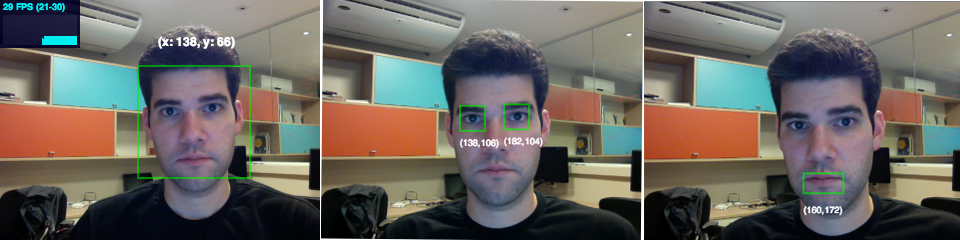
\includegraphics[width=\linewidth]{chapters/evaluation/viola_overview.png}
  \caption{Library implementation of Viola Jones using different training datas for detecting faces, eyes and mouth.}
  \label{figure:viola_overview}
\end{figure}

\begin{figure}[!htb]
  \centering
  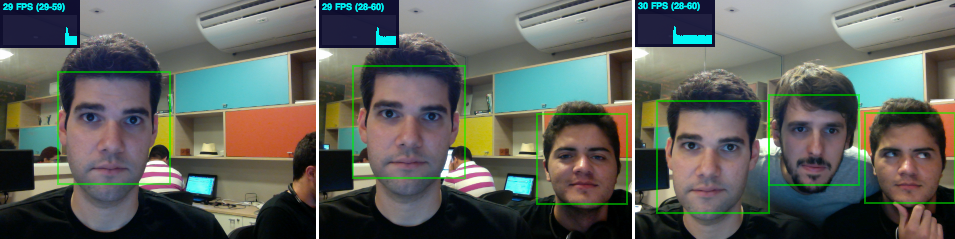
\includegraphics[width=\linewidth]{chapters/evaluation/viola.png}
  \caption{Library implementation of Viola Jones detecting multiple faces inside the real-time limit of 25 FPS.}
  \label{figure:viola_multiple_faces}
\end{figure}

Augmented reality and tracking applications for advertising and entertainment are gaining more space on the web enviroment. The media used in this kind of application needs to be as appealing as possible in order to catch consumers' attention, thus detecting faces, or augmenting the scene with objects are attractive possibilities. In order to demonstrate that concept, a simple chat application was created. In this chat application, while talking in real-time, the users could augment their faces with objects, such as a fake glass with mustache. In order to extract the users eyes coordinates Viola Jones was used. Listing \ref{lst:viola} shows the simplified JavaScript API provided by \textit{tracking.js} in order to extract eyes coordinates and draw the image. The fake glasses are positioned over $x$ and $y$ coordinates on the canvas axis based on the extracted values. Figure \ref{figure:viola_glass_face} demonstrates the described example.

\begin{figure}[!htb]
  \centering
  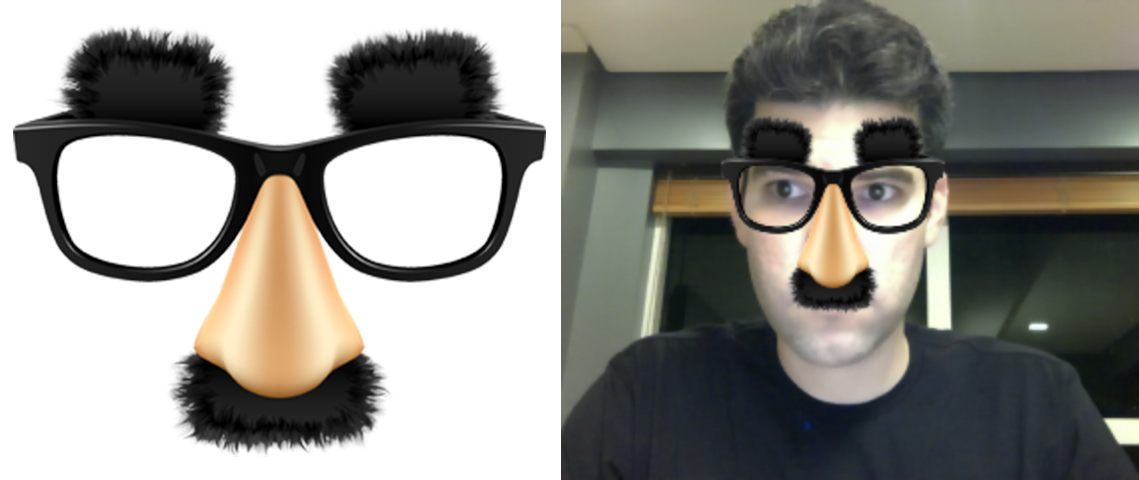
\includegraphics[width=380pt]{chapters/evaluation/viola_glass_face.png}
  \caption{Augmenting users faces with objects using \textit{tracking.js} Viola Jones eyes detection.}
  \label{figure:viola_glass_face}
\end{figure}

\begin{lstlisting}[language=C++,label={lst:viola},caption=Example of \textit{tracking.js} API of augmenting users faces with objects using Viola Jones eyes detection.]
  var img = new Image();
  img.src = 'img/glasses.png';
  var videoCamera = new tracking.VideoCamera();
  videoCamera.track({
      type: 'human',
      data: 'frontal_face',
      onFound: function(track) {
          videoCamera.canvas.context.drawImage(img, track[0].x, track[0].y, track[0].size, track[0].size);
      }
  });
\end{lstlisting}

% subsubsection discussion (end)

\subsubsection{FPS} % (fold)
\label{subsub:evaluation:results:rapid_object_detection:fps}

The United Kingdom popular video format known as Phase Alternating Line (PAL) \cite{PAL1962} defines that real time video is represented by 25 FPS, therefore this value is used to define whether the tests can or cannot be considered real-time. On Figure \ref{figure:viola_fps}, the Viola Jones implementation were tested with different numbers of detected faces. Fifteen faces were gradually added, for each addition the FPS average was recorded. Note that, until five faces detected the web implementation still runs inside the real-time limit defined by PAL \cite{PAL1962}.

\begin{figure}[!htb]
  \centering
    \begin{tikzpicture}
    \begin{axis}[
        enlarge x limits=0.03,
        minor tick num=1,
        xlabel=Number of detected faces,
        ylabel=Frames per second (FPS)]

        \addplot[wblue,mark=x] coordinates {
             (1,30)
             (2,29)
             (3,30)
             (4,27)
             (5,25)
             (6,20)
             (7,17)
             (8,16)
             (9,16)
             (10,15)
             (11,15)
             (12,13)
             (13,11)
             (14,9)
             (15,8)
         };

         \draw [red] ({rel axis cs:0,0}|-{axis cs:15,25}) -- ({rel axis cs:1,0}|-{axis cs:15,25}) node [pos=0.0, above] {};
    \end{axis}
    \end{tikzpicture}
   \caption{Library implementation of Viola Jones tested with different numbers of detected faces.}
   \label{figure:viola_fps}
\end{figure}

% subsubsection fps (end)

\subsubsection{Oclusion Robustness} % (fold)
\label{subsub:evaluation:results:rapid_object_detection:occlusion_robustness}

Viola Jones implementation of \textit{tracking.js} shows good results for partial occlusions. Figure \ref{figure:viola_occlusion} demonstrates occlusions variations that still allows the face to be detected.

\begin{figure}[!htb]
  \centering
  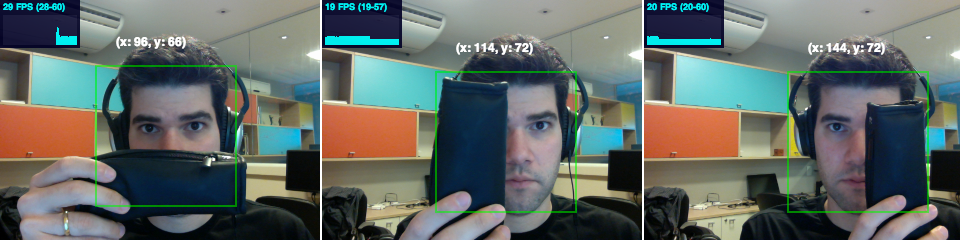
\includegraphics[width=\linewidth]{chapters/evaluation/viola_occlusion.png}
  \caption{Library implementation of Viola Jones partial occlusion robustness.}
  \label{figure:viola_occlusion}
\end{figure}

% subsubsection occlusion_robustness (end)

% subsection rapid_object_detection (end)

\subsection{Markerless Tracking Algorithm} % (fold)
\label{sec:evaluation:results:markerless_tracking_algorithm}

\subsubsection{Matching Robustness} % (fold)
\label{subsub:evaluation:results:markerless_tracking_algorithm:matching_robustness}

Lorem ipsum dolor sit amet, consectetur adipisicing elit.

% subsubsection matching_robustness (end)

\subsubsection{Oclusion Robustness} % (fold)
\label{subsub:evaluation:results:markerless_tracking_algorithm:occlusion_robustness}

Lorem ipsum dolor sit amet, consectetur adipisicing elit.

% subsubsection occlusion_robustness (end)

% subsection markerless_tracking_algorithm (end)

\subsection{Color Tracking Algorithm} % (fold)
\label{sec:evaluation:results:color_tracking_algorithm}

\subsubsection{Matching Robustness} % (fold)
\label{subsub:evaluation:results:color_tracking_algorithm:matching_robustness}

Lorem ipsum dolor sit amet, consectetur adipisicing elit.

% subsubsection matching_robustness (end)

\subsubsection{Oclusion Robustness} % (fold)
\label{subsub:evaluation:results:color_tracking_algorithm:occlusion_robustness}

Lorem ipsum dolor sit amet, consectetur adipisicing elit.

% subsubsection occlusion_robustness (end)

\subsubsection{FPS} % (fold)
\label{subsub:evaluation:results:color_tracking_algorithm:fps}

Lorem ipsum dolor sit amet, consectetur adipisicing elit.

% subsubsection fps (end)

% subsection color_tracking_algorithm (end)

% section results (end)

% chapter evaluation (end)